\chapter{Environnement de Développement}
\label{chap:Chapter 2 title}
\section*{Introduction}


\hspace{16pt}Dans ce chapitre, nous explorons l'environnement de développement utilisé pour ce projet. Un environnement de développement bien choisi est crucial pour assurer une productivité élevée, une gestion efficace du code et une collaboration harmonieuse entre les membres de l'équipe. Nous détaillerons les outils et technologies spécifiques qui ont été adoptés, tels que le système d'exploitation, les éditeurs de texte, les terminaux, et les systèmes de contrôle de version.


\pagebreak


\section{Système d'Exploitation: Arch Linux (BTW)}

\hspace{16pt}Pour le développement de ce projet, j'ai choisi d'utiliser Arch Linux comme système d'exploitation principal. Arch Linux est une distribution Linux réputée pour sa simplicité, sa flexibilité et son approche "rolling release", ce qui permet d'avoir toujours les dernières versions des logiciels et des bibliothèques. Ma décision d'opter pour Arch Linux a été motivée par plusieurs facteurs, notamment:

\subsection{Simplicité et Contrôle}

\hspace{16pt}Arch Linux suit la philosophie "Keep It Simple, Stupid" (KISS), offrant un contrôle total sur l'installation et la configuration du système. Cette approche minimaliste m'a permis de créer un environnement de développement sur mesure, en installant uniquement les packages et les outils nécessaires pour le projet, sans superflu ni bloatware.

\subsection{Documentation Complète}

\hspace{16pt}L'Arch Wiki, la documentation officielle d'Arch Linux, est une ressource exhaustive qui couvre une large gamme de sujets. Cette documentation détaillée m'a été particulièrement utile pour la configuration du système, la résolution de problèmes techniques et l'apprentissage de nouvelles compétences liées à Linux.

\subsection{Mise à Jour Continue}

\hspace{16pt}Grâce à son modèle "rolling release", Arch Linux fournit les versions les plus récentes des logiciels, ce qui est crucial pour un développement moderne et efficace. En ayant toujours accès aux dernières fonctionnalités et aux correctifs de sécurité, j'ai pu travailler avec des outils à jour et bénéficier des dernières avancées technologiques.

\subsection{Communauté Active}

\hspace{16pt}La communauté Arch Linux est réputée pour son dynamisme et son engagement. Les forums, les canaux IRC et d'autres plateformes de discussion offrent un soutien continu, des conseils pratiques et des solutions aux problèmes rencontrés. Cet écosystème vibrant a contribué à enrichir mon expérience avec Arch Linux et à résoudre rapidement les défis rencontrés.


\section{Éditeurs de texte: (Neo)Vim}

\hspace{16pt}Pour le développement de ce projet, j'ai choisi d'utiliser Neovim comme éditeur de texte principal. Neovim est une version améliorée de Vim, un éditeur de texte puissant et hautement configurable, largement utilisé dans la communauté des développeurs. Ma décision d'opter pour Neovim a été motivée par plusieurs facteurs, notamment:

\subsection{Inspiration}

\hspace{16pt}Je me suis inspiré de créateurs de contenu renommés tels que ThePrimeagen, TJ DeVries, Typecraft, et Dreams of Code, qui partagent leur expertise et leurs astuces sur Neovim à travers des tutoriels, des vidéos et des configurations. Leur maîtrise de Neovim et leurs conseils ont été une source d'inspiration et d'apprentissage pour moi, m'encourageant à explorer davantage les fonctionnalités avancées de Neovim et à personnaliser mon propre environnement de développement.

\subsection{Configuration Personnalisée}

\hspace{16pt}Ma configuration Neovim a été entièrement personnalisée avec plus de 1100 lignes de code. Cette configuration comprend des réglages de base, des raccourcis clavier, des plugins, des thèmes et des intégrations avec d'autres outils de développement. En m'appuyant sur les bonnes pratiques et les astuces partagées par la communauté, j'ai pu créer un environnement de développement optimisé et ergonomique, adapté à mes besoins spécifiques et à mon flux de travail.

\subsection{Avantages de Neovim}

\begin{itemize}
  \item \textbf{Performance: }Neovim est conçu pour offrir des performances supérieures à Vim, notamment en termes de vitesse de chargement des fichiers et de réactivité des commandes.
  \item \textbf{Extensibilité: }La structure modulaire de Neovim permet d'ajouter facilement des fonctionnalités supplémentaires via des plugins et des scripts Lua, offrant ainsi une grande flexibilité et une adaptabilité aux besoins changeants du développement logiciel.
  \item \textbf{Communauté Active: }La communauté Neovim est dynamique et engagée, offrant un soutien continu, des mises à jour fréquentes et des contributions constantes à l'écosystème Neovim, ce qui garantit un développement continu et une évolution constante de l'éditeur.
  
\end{itemize}


\section{Terminal: Alacritty avec Zsh}

\hspace{16pt}Pour le développement de ce projet, j'ai utilisé Alacritty comme terminal principal, associé à Zsh comme shell par défaut. Alacritty est un émulateur de terminal GPU-accelerated écrit en Rust, connu pour sa réactivité et ses performances élevées. Rust est un langage de programmation moderne qui offre à la fois la sécurité du code et des performances exceptionnelles, ce qui en fait un choix idéal pour les applications sensibles aux performances comme Alacritty. Cette combinaison a été choisie pour améliorer mon flux de travail et ma productivité, et elle a été enrichie par plusieurs utilitaires et configurations personnalisées:

\subsection{Alacritty}

\hspace{16pt}Alacritty a été choisi pour sa légèreté et sa rapidité. Étant un émulateur de terminal écrit en Rust, Alacritty offre une expérience fluide et réactive, ce qui est essentiel pour un développement efficace. Ses principaux avantages sont:

\begin{itemize}
  \item \textbf{Performances élevées: }Alacritty est conçu pour être rapide, avec un temps de démarrage minimal et une réponse instantanée aux commandes.
  \item \textbf{Langage de Programmation Rust: }Alacritty est écrit en Rust, un langage de programmation moderne qui offre à la fois la sécurité du code et des performances exceptionnelles.
  \item \textbf{Personnalisable: }Alacritty offre de nombreuses options de personnalisation, notamment la possibilité de configurer les raccourcis clavier, les thèmes et les polices.
\end{itemize}

\subsection{Zsh}

\hspace{16pt}Zsh a été utilisé comme shell interactif principal, enrichi par une configuration personnalisée comprenant plusieurs plugins et utilitaires pour améliorer l'expérience utilisateur. Quelques éléments notables de cette configuration sont:

\begin{itemize}
  \item \textbf{Oh My Zsh: }J'ai utilisé Oh My Zsh, un framework de gestion de configuration Zsh, pour faciliter l'installation et la gestion des plugins et des thèmes.
  \item \textbf{Plugins Zsh: }J'ai intégré plusieurs plugins Zsh, tels que zsh-syntax-highlighting, zsh-completions, zsh-autosuggestions, et Aloxaf/fzf-tab, pour améliorer la syntaxe en surbrillance, la complétion automatique, et l'expérience de suggestion de commandes.
  \item \textbf{Zsh Theme personnalisé: }J'ai implémenté un thème Zsh personnalisé, adapté à mes préférences et à mon flux de travail, pour afficher des informations utiles telles que le répertoire de travail actuel, le statut du git, et d'autres informations système.
\end{itemize}

\subsection{Outils supplémentaires}

\hspace{16pt}En plus d'Alacritty et Zsh, j'ai utilisé plusieurs autres utilitaires pour améliorer mon flux de travail:

\begin{itemize}
  \item \textbf{Tmux: }Tmux a été utilisé pour la gestion des sessions et la possibilité de diviser l'écran en plusieurs panneaux. Cela m'a permis de travailler de manière plus efficace en ayant plusieurs terminaux ouverts simultanément pour différentes tâches.
  \item \textbf{Fzf: }Fzf a été utilisé pour la recherche rapide et interactive dans les fichiers, les historiques de commandes, et d'autres listes de données.
  \item \textbf{Zoxide: }Zoxide a été utilisé pour la navigation rapide dans le système de fichiers en se basant sur les répertoires les plus fréquemment utilisés.
  \item \textbf{Scripts Bash personnalisés: }J'ai écrit plusieurs scripts Bash personnalisés pour automatiser des tâches répétitives et simplifier les opérations courantes dans mon environnement de développement.
\end{itemize}


\section{Contrôle de Version: Git et GitHub}

\hspace{16pt}Pour la gestion du code source de ce projet, j'ai utilisé Git comme système de contrôle de version et GitHub comme plateforme d'hébergement et de collaboration. Git est un système de contrôle de version distribué largement utilisé, conçu pour suivre les modifications apportées au code source tout au long du développement d'un projet. GitHub, quant à lui, est une plateforme de développement collaboratif qui permet aux développeurs de partager leur code, de travailler en équipe et de contribuer à des projets open source. Voici quelques aspects de mon utilisation de Git et GitHub dans ce projet:

\subsection{Git}

\begin{itemize}
  \item \textbf{Gestion des Versions: }Git a été utilisé pour suivre l'évolution du code source tout au long du développement du projet. J'ai créé des commits réguliers pour enregistrer les modifications apportées au code et maintenir un historique clair et organisé.
  \item \textbf{Branches: }J'ai utilisé des branches Git pour travailler sur des fonctionnalités isolées et des correctifs de bugs sans perturber le code principal. Les branches m'ont permis de développer de manière collaborative tout en maintenant la stabilité du code.
  \item \textbf{Fusion (Merge): }Une fois les fonctionnalités développées et testées, j'ai fusionné les branches de développement dans la branche principale (main). Cette fusion a consolidé les modifications et intégré les nouvelles fonctionnalités dans le code principal du projet.
\end{itemize}

\begin{figure}[H] 
    \centering
    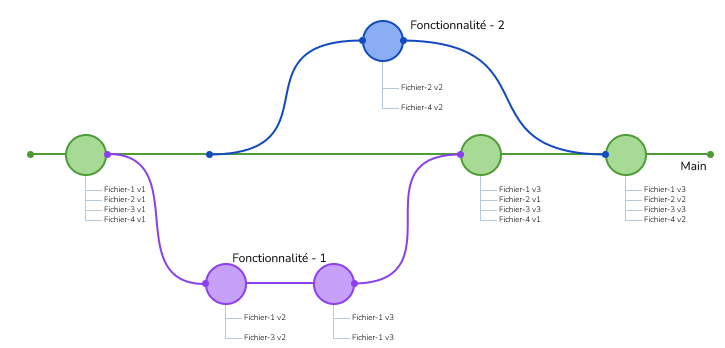
\includegraphics[width=18cm]{Figures/Git.png}
    \caption{Flux d'ajout des fonctionnalités en Git}
\end{figure}

%[width=7cm] you control the size of the image. other options include: 
%[height=7cm] or [scale=0.5] (means half the size of the original image)

\subsection{GitHub}

\begin{itemize}
  \item \textbf{Hébergement du Code: }J'ai hébergé le code source du projet sur GitHub, ce qui m'a permis de le partager facilement avec mes collaborateurs et mon encadrant.
  \item \textbf{Suivi des Problèmes (Issues): }J'ai utilisé la fonctionnalité des Issues sur GitHub pour suivre les tâches, les bogues et les demandes de fonctionnalités tout au long du développement du projet. Les Issues ont permis une communication efficace entre les membres de l'équipe et ont contribué à une gestion transparente des problèmes.
  \item \textbf{Pull Requests (Demandes de Tirage): }Pour intégrer les modifications dans le code principal du projet, j'ai créé des Pull Requests sur GitHub. Les Pull Requests ont facilité la révision du code par les pairs, les tests d'intégration et les validations avant la fusion finale.
\end{itemize}

\begin{figure}[H] 
    \centering
    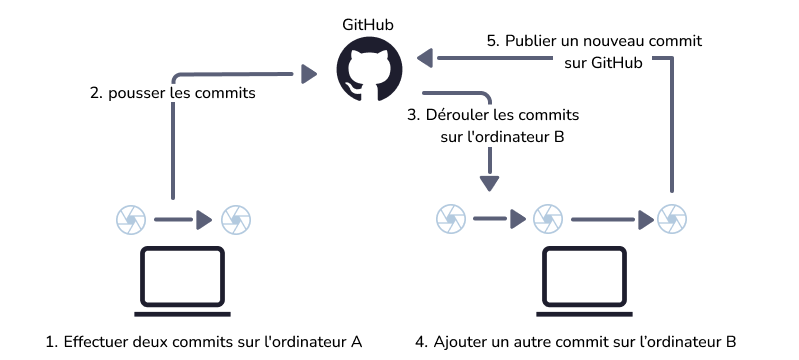
\includegraphics[width=18cm]{Figures/github.png}
    \caption{Collaborer sur github}
\end{figure}

\section{Autres Outils}

\subsection{\LaTeX}

\hspace{16pt}Pour la rédaction du rapport de ce projet, j'ai choisi d'utiliser \LaTeX, un système de composition de documents largement utilisé dans le domaine académique et technique pour sa capacité à produire des documents de haute qualité typographique. \LaTeX\xspace offre de nombreux avantages pour la rédaction de rapports techniques, notamment:

\begin{itemize}
  \item \textbf{Typographie de haute qualité: }\LaTeX\xspace produit des documents avec une typographie professionnelle et esthétique, offrant un rendu précis des symboles mathématiques, des formules, des tableaux et des graphiques.
  \item \textbf{Gestion avancée des références: }\LaTeX\xspace simplifie la gestion des références croisées, des citations bibliographiques et des tableaux des matières, ce qui facilite l'organisation et la navigation dans le rapport.
  \item \textbf{Séparation du contenu et de la mise en page: }\LaTeX\xspace permet de séparer le contenu du document de sa mise en page, ce qui facilite la modification et la réorganisation du contenu sans affecter la présentation visuelle.
\end{itemize}


\subsection{Postman}

\hspace{16pt}Postman a été un outil essentiel dans le processus de développement de l'API pour notre projet. En tant que plateforme de collaboration pour le développement d'API, Postman nous a permis de tester facilement les points de terminaison de notre API RESTful. Avec Postman, nous avons pu envoyer des requêtes HTTP, inspecter les réponses, et valider le comportement de notre API à différentes étapes du développement. L'interface conviviale de Postman nous a également permis de partager nos collections d'API avec d'autres membres de l'équipe et de collaborer efficacement sur les tests et les validations. En résumé, Postman a grandement facilité le processus de développement et de test de notre API, contribuant ainsi à la qualité et à la fiabilité de notre solution logicielle.


\subsection{Eraser}

\hspace{16pt}Eraser a été un élément essentiel de notre processus de conception pour visualiser l'architecture et le flux de notre application. Voici comment nous avons utilisé cet outil:

\begin{itemize}
  \item \textbf{Création de Diagrammes: }Eraser nous a permis de créer des diagrammes de classe, des diagrammes de séquence et d'autres types de schémas pour représenter les différents aspects de notre application.
  \item \textbf{Personnalisation: }Nous avons bénéficié d'une large gamme d'outils et de fonctionnalités offerts par Eraser, nous permettant ainsi de personnaliser nos diagrammes selon nos besoins spécifiques et de les rendre aussi clairs et informatifs que possible.
  \item \textbf{Collaboration: }L'interface intuitive d'Eraser et sa capacité à exporter des diagrammes dans divers formats ont facilité la collaboration au sein de l'équipe. Nous avons pu partager nos diagrammes avec les membres de l'équipe et les parties prenantes pour recueillir des commentaires et assurer une compréhension commune du système.
\end{itemize}


\subsection{Figma}

\hspace{16pt}Figma a été un outil polyvalent dans notre processus de conception, nous permettant de créer à la fois des diagrammes détaillés et des présentations visuellement attrayantes. Voici comment nous l'avons utilisé:

\begin{itemize}
  \item \textbf{Création de Diagrammes: }Comme Eraser, Figma nous a permis de créer des diagrammes de classe, des diagrammes de séquence et d'autres types de schémas pour représenter l'architecture et le flux de notre application. Nous avons bénéficié d'une interface conviviale et d'outils intuitifs pour réaliser ces diagrammes avec précision.
  \item \textbf{Présentations Visuelles: }En plus de la création de diagrammes, Figma a également été utilisé pour créer des présentations visuellement attrayantes. Nous avons pu intégrer des diagrammes, des maquettes d'interface utilisateur et d'autres éléments visuels dans nos présentations pour communiquer efficacement nos idées et nos concepts.
\end{itemize}

\newpage

\section*{Conclusion}


\hspace{16pt}Ce chapitre a couvert les différents composants de l'environnement de développement, incluant Arch Linux comme système d'exploitation, Neovim pour l'édition de texte, Alacritty comme terminal, et Git pour le contrôle de version. Chaque choix a été justifié par ses avantages spécifiques pour le projet.
